\section{Пример: данные о пространственном восприятии}

Следующий пример, основанный на данных о пространственном восприятии, показывает необходимость улучшения процентильного метода и метода бутстреп-t. Каждый из двадцати шести детей с неврологическими дефектами проходил два теста на пространственное восприятие, тест <<A>> и тест <<B>>. Эти данные показаны в таблице 14.1 и представлены графически на рис. 14.1.

\noindent
\begin{center}
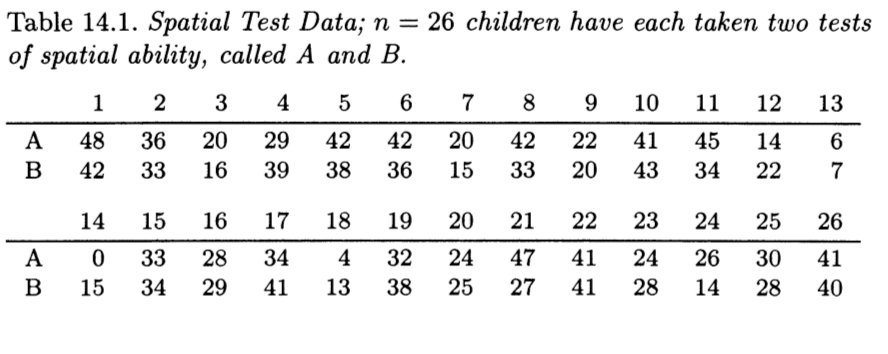
\includegraphics[width=0.9\linewidth]{14/t141.png}
\end{center}
\setcounter{table}{1}

Предположим, что мы хотим найти 90\% доверительный интервал для $\theta = \text{var} (A)$, дисперсии результата теста <<A>>.

Оценка $\theta$ по методу подстановки основана на $n=26$ парах $x_i = (A_i, B_i)$ из таблицы 14.1.
\begin{equation}
	\thetahat = \summ{i = 1}{n} (A_i - \bar A)^2/n = 171.5, \qquad (\hat A = \summ{i = 1}{n} A_i/n)
\end{equation}
\setcounter{equation}{1}
Следует заметить, что это немного меньше обычной несмещенной оценки~$\theta$,
\begin{equation}
	\bar\theta = \summ{i = 1}{n} (A_i - \bar A)^2/(n-1) = 178.4
\end{equation}
\setcounter{equation}{2}
Оценка методом подстановки $\thetahat$ смещена вниз. Метод $\bca$ автоматически делает поправку на смещение в оценке по методу подстановки, что является одним из его достоинств перед процентильным методом.\footnote{Для рассуждений в этой части, а также для алгоритмов \texttt{bcanon} и \texttt{abcnon}, предполагаем, что статистика имеет форму $\thetahat = t(\hat F)$ (получена методом подстановки)}
Гистограмма 2000 бутстреп репликаций $\thetahat^*$ показана на левой панели рисунка 14.2. Репликации получены таким же образом, как и в случае рисунка 6.1: если $\mathbf x = (\xes{26})$ представляет из себя исходный набор данных таблицы 14.1, где $x_i = (A_i,B_i)$, $\ies{26}$, тогда бутстреп выборка $\mathbf x^* = (\xest{26})$ есть случайная выборка размера 26 с возвращением из набора $\{\xes{26}\}$; бутстреп репликация $\thetahat^*$ есть дисперсия А компонент $\bf x^*$, где $x_i^* = (A_i^*, B_i^*),$
\begin{equation}
	\thetahat = \summ{i = 1}{n} (A_i^* - \bar A^*)^2/n, \qquad (\hat A^* = \summ{i = 1}{n} A_i^*/n).
\end{equation}
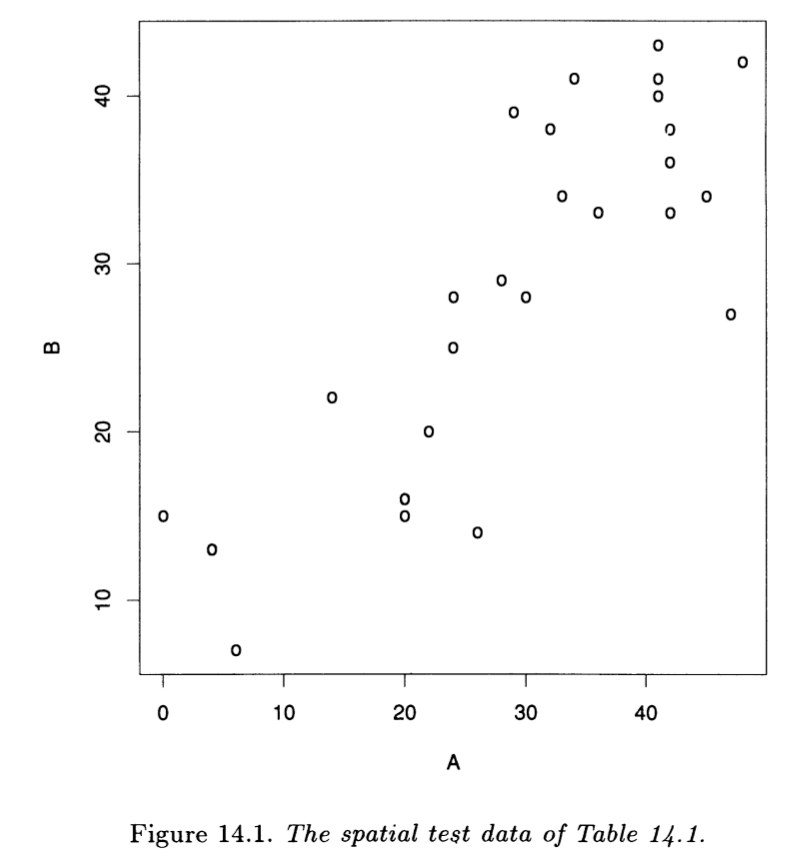
\includegraphics[width=0.85\linewidth]{14/f141.png}
\newline
$B = 2000$ бутстреп выборок $\mathbf x$ дают 2000 бутстреп репликаций $\thetahat^*$ на рис.14.2.\footnote{легко проверить, что нам не нужны вторые компоненты $x_i^*$ для этих вычислений} Это так называемые \textit{непараметрические} бутстреп репликации, которые мы уже рассматривали в предыдущих частях. Далее мы также обсудим \textit{параметрические} бутстреп репликации, а именно предположим нормальную модель для данных. Согласно обозначениям главы 6, непараметрическая бутстреп выборка генерируется случайным выбором из $\widehat F$,
\begin{equation}
	\widehat F \rightarrow \mbf x^* = (\xest{n}),
\end{equation}
\setcounter{equation}{4}
где $\what F$ есть эмпирическая функция распределения, для которого вероятность каждого из $x_i$ равна $1/n$.

В верхней части таблицы 14.2 показаны пять различных приближенных $90\%$ непараметрических доверительных интервалов для $\theta$: 
\begin{itemize}
	\item стандартный интервал $\what \theta \pm 1.645\what \sigma$;
	\item бутстреп оценка стандартной ошибки;
	\item процентильный интервал $(\what \theta^{*(0.05)}, \what \theta^{*(0.95)})$, построенный на основе левой гистограммы на рис. 14.2;
	\item $\bca$ и $\abc$ интервалы, которые обсуждаются в следующих двух разделах;
	\item бутстреп-t интервалы из главы 12. 
\end{itemize}

\noindent
\begin{center}
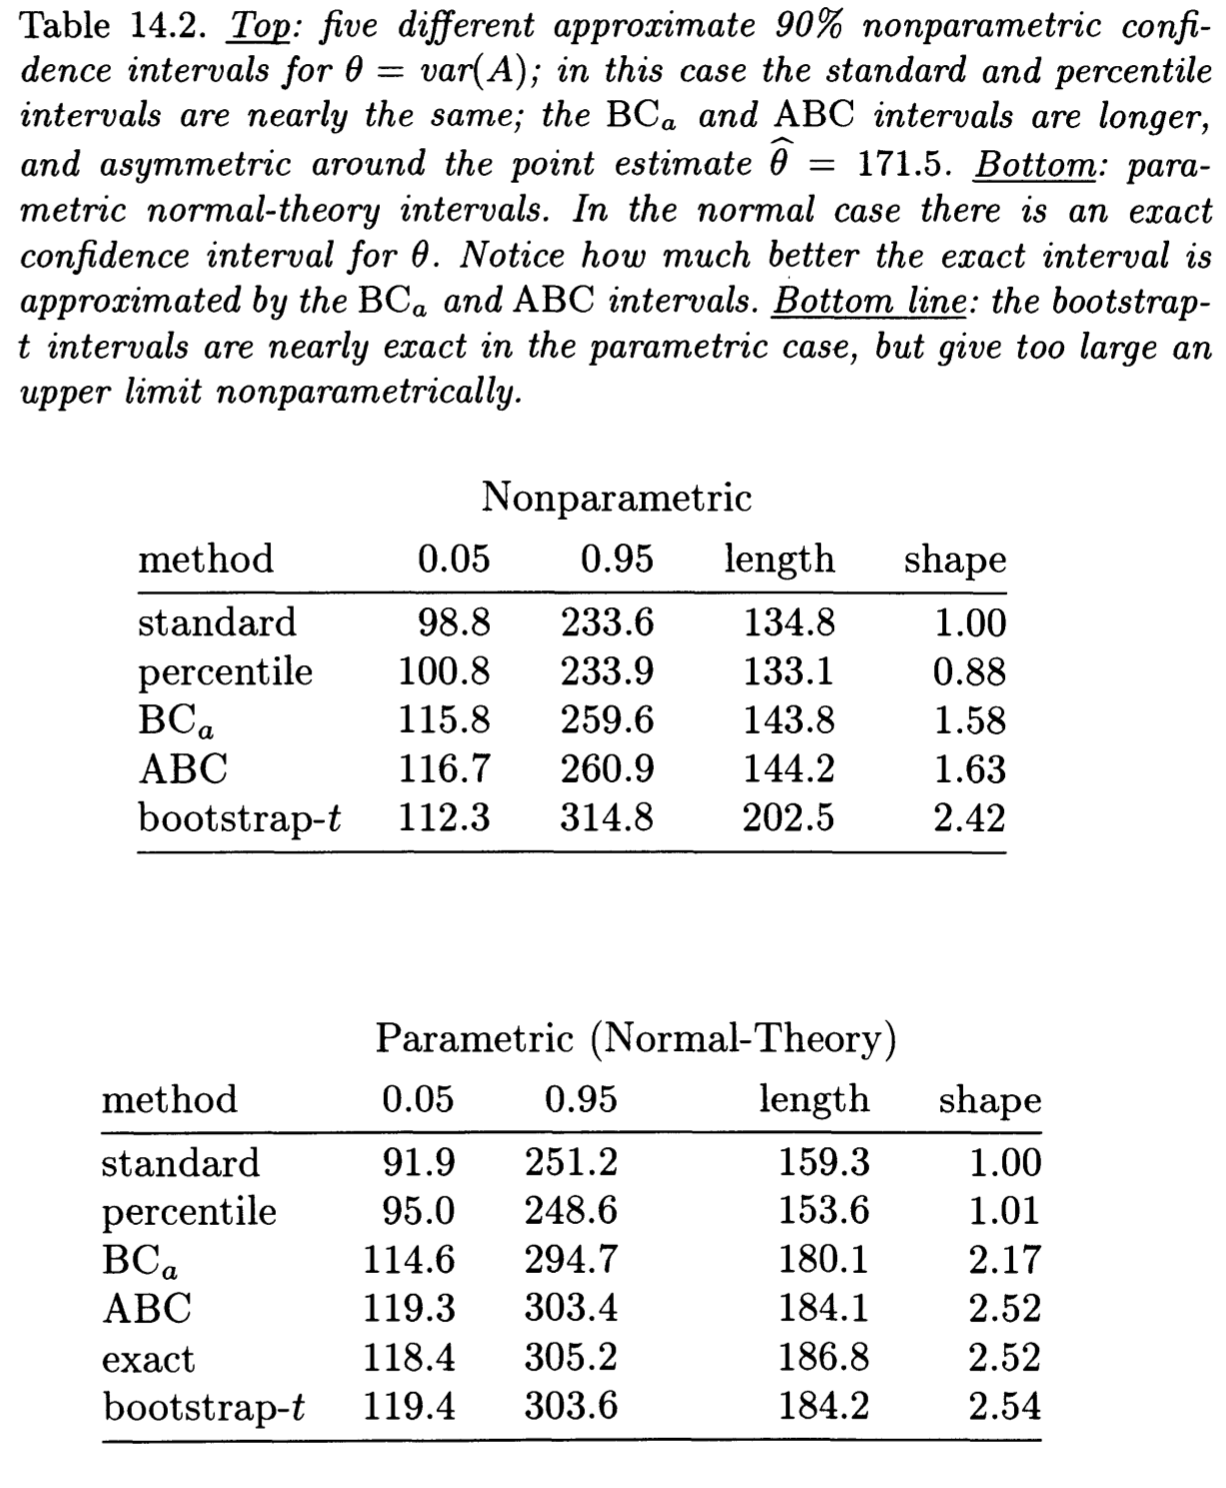
\includegraphics[width=0.9\linewidth]{14/t142.png}
\end{center}
\setcounter{table}{2}
Каждый из интервалов $(\what \theta_\tx{lo}, \what \theta_\tx{up})$ определяется своей длиной и формой (shape):
\begin{equation}
	\tx{length} = \what \theta_\tx{up} - \what \theta_\tx{lo}, \qquad \tx{shape} = \frac{\what{\theta}_\tx{up} - \what{\theta}}{\what{\theta} - \what{\theta}_\tx{lo}}.
\end{equation}
<<Форма>> есть показатель асимметричности интервала относительно оценки $\what \theta$. Показатель формы больший, чем 1, означает, что расстояние между $\what{\theta}$~и~$\what{\theta}_\tx{up}$ больше, чем расстояние между $\what{\theta}$ и $\what{\theta}_\tx{lo}$. Стандартные интервалы симметричны относительно $\what \theta$, откуда $\tx{shape} = 1$ по определению. Точные интервалы, когда они существуют, чаще всего оказываются асимметричными. Построенные стандартные интервалы оказываются ошибочными во-многом из-за их <<врожденной>> симметрии. 

Для рассматриваемого набора данных стандартные и процентильные интервалы практически совпадают. Оба несколько отличаются от $\bca$ и $\abc$ интервалов, которые оказались более длинными и асимметричными вправо относительно $\what \theta$. Общий результат, приведенный в разделе 13.2, говорит о том, что интервалы $\bca$ и $\abc$ лучше, однако мы не можем утверждать об этом однозначно, так как для таких сравнений не существует <<золотого стандарта.>>

В то же время, мы можем получить <<золотой стандарт>>, если рассмотрим задачу оценивания $\tx{var} (A)$ в рамках параметрического подхода (предположив гауссовость\footnote{На самом деле, не похоже, что исходные данные распределены нормально. Однако это не запрещает провести сравнительный анализ методов, аппроксимирующих точный интервал \textit{в предположении}, что данные распределены нормально. Все же, если сравнивать параметрические и непараметрические интервалы, то последние оказываются более предпочтительными для данного набора данных.}). Для этого мы предположим, что результаты тестов $x_i = (A_i, B_i)$ есть случайная выборка из двумерного нормального распределения $F_\tx{norm},$
\begin{equation}
  F_\tx{norm} \rightarrow \mbf x = (\xes{n}).
\end{equation}
При выбранном параметрическом подходе мы можем построить точный доверительный интервал для $\theta = \tx{var} (A)$. %См. задачу 14.4
Этот интервал, названный <<точным>> (\textit{exact}) в таблице 14.2, является <<золотым стандартом>> для оценки различных приближенных интервалов в параметрических условиях.
Выборка гауссового параметрического бутстрепа получается генерацией выборок из двумерного нормального распределения $\what F_\tx{norm}$, которое наилучшим образом соответствует данным $\mbf x$ вместо эмпирического распределения $\what F$, то есть
\begin{equation}
  \what F_\tx{norm} \rightarrow \mbf x^* = (\xest{n}).
\end{equation}
%См. задачу 14.3.
Получив $\mbf x^*$, бутстреп репликация $\what \theta^*$ будет равна 
$$
\summ{1}{n} (A_i^* - \bar A^*)^2/n,
$$
как в (14.3). 

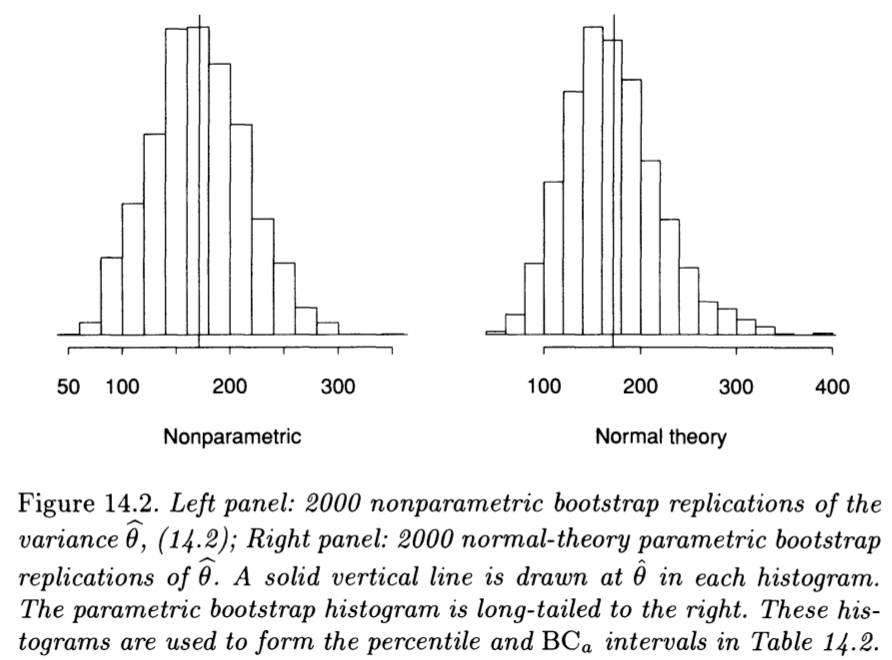
\includegraphics[width=0.85\linewidth]{14/f142.png}
\newline
\noindent Правая гистограмма на рис. 14.2 --- гистограмма 2000 репликаций параметрического бутстрепа. Если сравнить ее с непараметрической версией, гистограмма \textit{normal theory} имеет длинный хвост справа, а также шире, при этом $\what \sigma = 47.1$, если сравнить со стандартной ошибкой в непараметрическом случае --- 41.0.

Если обратить внимание на нижнюю часть таблицы 14.2, то можно увидеть, что интервалы по методам $\bca$ и $\abc$ оказываются близкими к точному <<золотому стандарту>>. И это не просто случайность или частный случай. На самом деле, теория бутстрепа, приведенная кратко в разделе 14.3, говорит о том, что мы можем ожидать успешные результаты от $\bca$ и $\abc$.

Бутстреп-t интервалы для $\theta$ показаны в нижних частях таблицы 14.2. Они основаны на 1000 бутстреп репликаций статистики (по аналогии с $t$-статистикой) $(\what \theta - \theta)/\what{\tx{se}}$, со знаменателем, <<взятым>> из стандартной статистической теории,
\begin{equation}
  \what{\tx{se}} = \left[ \frac{U_4 - U_2^2}{26}  \right]^{1/2} \qquad (U_h = \summ{i = 1}{26} (A_i - \bar A)^h/26).
\end{equation}

Результирующие интервалы, как в (12.19), оказываются практически точными в случаях нормальной теории. Однако верхний предел непараметрического интервала кажется слишком большим, хотя об этом сложно утверждать в отсутствии непараметрического <<золотого стандарта>>. На данном уровне развития метод бутстреп-t не может быть рекомендован к использованию в непараметрической постановке.

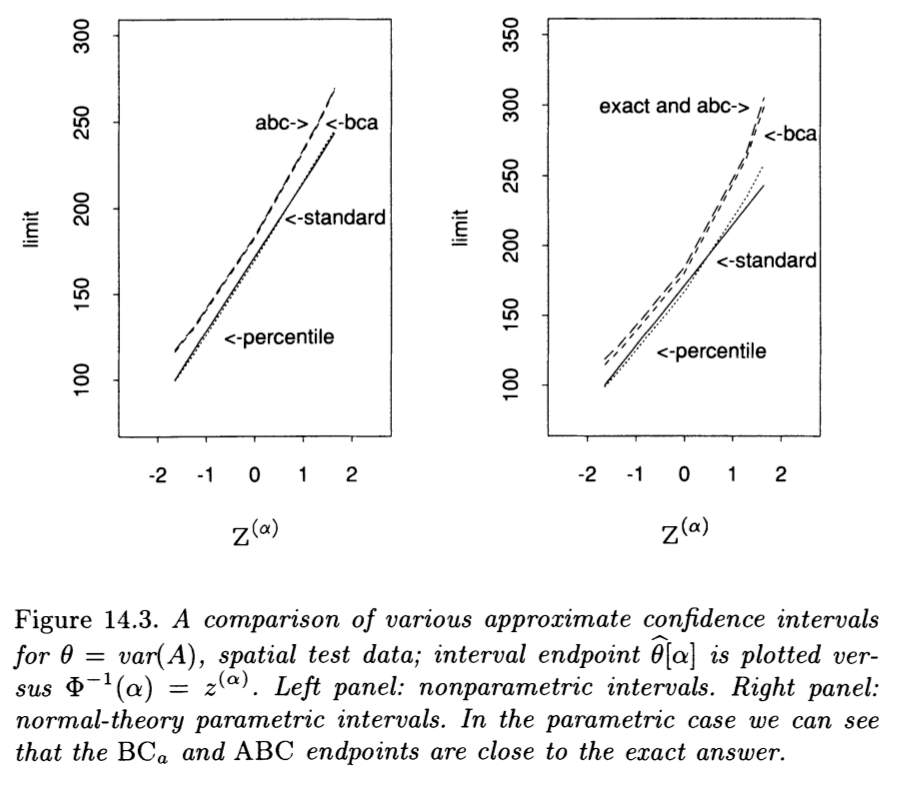
\includegraphics[width=0.85\linewidth]{14/f143.png}
\newline


